%\documentclass[aps,twocolumn,longbibliography,english,superscriptaddress]{revtex4-1}
\documentclass{article}
\usepackage{iclr2021_conference}
%\documentclass[a4paper,superscriptaddress,11pt]{article}
\pdfoutput=1
\usepackage[colorlinks=true,urlcolor=blue,citecolor=blue,linkcolor=blue]{hyperref}
\usepackage[english]{babel}
\usepackage[utf8]{inputenc}
\usepackage[T1]{fontenc}
\usepackage{amssymb}
\usepackage{tabularx}
\usepackage{quoting}
\usepackage{upquote}
\usepackage{subcaption}
\usepackage{multicol}
\usepackage[framemethod=TikZ]{mdframed}
\usepackage{wrapfig}
%\usepackage{caption}
%\usepackage[plain]{algorithm}
\usepackage[linesnumbered, ruled, vlined]{algorithm2e}
\usepackage{algpseudocode}
\usepackage{rotating}
%\usepackage{cite}
\usepackage{booktabs}
%\usepackage{unicode-math}
%\usepackage{algorithm}% http://ctan.org/pkg/algorithm
%\usepackage{algpseudocode}% http://ctan.org/pkg/algpseudocode
\usepackage{xcolor}% http://ctan.org/pkg/xcolor
\makeatletter
\newsavebox{\@brx}
\newcommand{\llangle}[1][]{\savebox{\@brx}{\(\m@th{#1\langle}\)}%
  \mathopen{\copy\@brx\kern-0.5\wd\@brx\usebox{\@brx}}}
\newcommand{\rrangle}[1][]{\savebox{\@brx}{\(\m@th{#1\rangle}\)}%
  \mathclose{\copy\@brx\kern-0.5\wd\@brx\usebox{\@brx}}}
\makeatother
\usepackage{bbm}
\usepackage{jlcode}
\usepackage{graphicx}
\usepackage{amsmath,color,amsthm}
\usepackage{mathrsfs}
\usepackage{float}
\usepackage[normalem]{ulem}
\usepackage{makecell}
\usepackage{indentfirst}
\usepackage{txfonts}
\usepackage[epsilon, tsrm, altpo]{backnaur}

\DeclareMathAlphabet{\mymathbb}{U}{BOONDOX-ds}{m}{n}
\newcommand{\listingcaption}[1]%
{%
\refstepcounter{lstlisting}\hfill%
Listing \thelstlisting: #1\hfill%\hfill%
}%
\newcolumntype{b}{X}
\newcolumntype{s}{>{\hsize=.7\hsize}X}
\usepackage{listings}
\lstset{
    language=Julia,
    basicstyle=\ttfamily\scriptsize,
    numberstyle=\scriptsize,
    % numbers=left,
    backgroundcolor=\color{gray!7},
    %backgroundcolor=\color{white},
    %frame=single,
    xleftmargin=2em,
    tabsize=2,
    rulecolor=\color{black!15},
    %title=\lstname,
    escapeinside={(*}{*)},
    breaklines=true,
    %breakatwhitespace=true,
    %framextopmargin=2pt,
    %framexbottommargin=2pt,
    frame=bt,
    extendedchars=true,
    inputencoding=utf8,
    columns=fullflexible,
    %escapeinside={(*@}{@*)},
}

\tolerance=1
\emergencystretch=\maxdimen
\hyphenpenalty=1000
\hbadness=1000

\makeatletter

%%%%%%%%%%%%%%%%%%%%%%%%%%%%%% User specified LaTeX commands.

%Journal reference.  Comma sets off: name, vol, page, year
\def\journal #1, #2, #3, 1#4#5#6{{\sl #1~}{\bf #2}, #3 (1#4#5#6) }
\def\pr{\journal Phys. Rev., }
\def\prb{\journal Phys. Rev. B, }
\def\prl{\journal Phys. Rev. Lett., }
\def\pl{\journal Phys. Lett., }
%\def\np{\journal Nucl. Phys., }


%%%%%%%%%%%%%%%%%%%%%%%%%%%%%%%%%%%%%%%%%%%%%%%%%%%%%%%%%%%%%%%%%%%%%%%%%%%%%%%%%%%%%%%%%%%%%%%%%%%%%%%%%%%%%%%%%%%%%%%%%%%%%%%%%%%%%%%%%%%%%%%%%%%%%%%%%%%%%%%%%%%%%%%%%%%%%%%%%%%%%%%%%%%%%%%%%%%%%%%%%%%%%%%%%%%%%%%%%%%%%%%%%%%%%%%%%%%%%%%%%%%%%%%%%%%%


%\usepackage{CJK}
%\usepackage[colorlinks, citecolor=blue]{hyperref}
\DeclareMathOperator*{\argmax}{arg\,max}

%%%%%% Shortcut related
\newcommand{\<}{\langle}
\renewcommand{\>}{\rangle}
\newcommand{\out}{{\vx^L}}
\newcommand{\inp}{{\vx^0}}
\newcommand{\cquad}{{{ }_{\quad}}}
\newcommand{\pluseq}{\mathrel{+}=}
\newcommand{\minuseq}{\mathrel{-}=}
\newcommand{\vx}{{\mathbf{x}}}
\newcommand{\vg}{{\mathbf{g}}}
\newcommand{\vp}{{\mathbf{p}}}
\newcommand{\vy}{{\mathbf{y}}}
\newcommand{\Var}{{\mathrm{Var}}}
\newcommand{\Mean}{{\mathrm{E}}}
\newcommand{\vvalue}{{\texttt{value}}}
\newcommand{\grad}{{\texttt{grad}}}
\newcommand{\parameter}{{\texttt{parameter}}}
%%%%%% Convention related
\newcommand{\SWAP}{{\rm SWAP}}
\newcommand{\CNOT}{{\rm CNOT}}
\newcommand{\bigO}{{\mathcal{O}}}
\newcommand{\X}{{\rm X}}
\renewcommand{\H}{{\rm H}}
\newcommand{\Rx}{{\rm Rx}}
\renewcommand{\v}[1]{{\bf #1}}
\newcommand{\dataset}{{\mathcal{D}}}
\newcommand{\wfunc}{{\psi}}
\newcommand{\SU}{{\rm SU}}
\newcommand{\UU}{{\rm U}}
\newcommand{\thetav}{{\boldsymbol{\theta}}}
\newcommand{\gammav}{{\boldsymbol{\gamma}}}
\newcommand{\thetai}{{\theta^\alpha_l}}
\newcommand{\Expect}{{\mathbb{E}}}
\newcommand{\Tr}{{\rm Tr}}
\renewcommand{\cite}[1]{{\citep{#1}}}
\newcommand{\etc}{{\it etc~}}
\newcommand{\etal}{{\it etal~}}
\newcommand{\xset}{\mathbf{X}}
\newcommand{\fl}{\texttt{fl}}
\newcommand{\pdata}{\mathbf{\pi}}
\newcommand{\q}{\mathbf{q}}
\newcommand{\epdata}{\mathbf{\hat{\pi}}}
\newcommand{\gammaset}{\boldsymbol{\Gamma}}
\newcommand{\ei}{{\mathbf{e}_l^\alpha}}
\newcommand{\vtheta}{{\boldsymbol{\theta}}}
\newcommand{\sigmag}{{\nu}}
\newcommand{\sigmai}[2]{{\sigma^{#2}_{#1}}}
\newcommand{\qi}[1]{{q^{\alpha_{#1}}_{#1}}}
\newcommand{\BAS}{Bars-and-Stripes}
\newcommand{\circled}[1]{\raisebox{.5pt}{\textcircled{\raisebox{-.9pt} {#1}}}}
\newcommand{\qexpect}[1]{{\left\langle #1\right\rangle}}
\newcommand{\expect}[2]{{\mathop{\mathbb{E}}\limits_{\substack{#2}}\left[#1\right]}}
\newcommand{\var}[2]{{\mathop{\mathrm{Var}}\limits_{\substack{#2}}\left(#1\right)}}
\newcommand{\pshift}[1]{{p_{\thetav+#1}}}
\newcommand{\upcite}[1]{\textsuperscript{\cite{#1}}}
\newcommand{\Eq}[1]{Eq.~(\ref{#1})}
\newcommand{\Fig}[1]{Fig.~\ref{#1}}
\newcommand{\Lst}[1]{Listing.~\ref{#1}}
\newcommand{\Tbl}[1]{Table~\ref{#1}}
\newcommand{\Sec}[1]{Sec.~\ref{#1}}
\newcommand{\App}[1]{Appendix~\ref{#1}}
\newcommand{\bra}[1]{\mbox{$\left\langle #1 \right|$}}
\newcommand{\ket}[1]{\mbox{$\left| #1 \right\rangle$}}
\newcommand{\braket}[2]{\mbox{$\left\langle #1 | #2 \right\rangle$}}
\newcommand{\tr}[1]{\mathrm{tr}\mbox{$\left[ #1\right]$}}

\newcommand{\ra}[1]{\renewcommand{\arraystretch}{#1}}

%%%%%% Comment related
\newcommand{\red}[1]{[{\bf  \color{red}{LW: #1}}]}
\newcommand{\xred}[1]{[{\bf  \color{red}{\sout{LW: #1}}}]}
\newcommand{\blue}[1]{[{\bf  \color{blue}{JG: #1}}]}
\newcommand{\violet}[1]{[{\bf  \color{violet}{MLS: #1}}]}
\newcommand{\green}[1]{[{\bf  \color{green}{TZ: #1}}]}
\newcommand{\xgreen}[1]{[{\bf  \color{green}{\sout{TZ: #1}}}]}
\newcommand{\xblue}[1]{[{\bf  \color{blue}{\sout{JG: #1}}}]}
\newcommand{\material}[1]{\iffalse[{\bf  \color{cyan}{Material: #1}}]\fi}
\newcommand{\orange}[1]{\iffalse[{\bf  \color{orange}{Jo: #1}}]\fi}

\newtheorem{theorem}{\textit{Branching Rule}}
\theoremstyle{definition}\newtheorem{definition}{\textit{Definition}}

\makeatother

\iclrfinalcopy
\begin{document}
\title{Solving the maximum independant set problem with einsum networks}

\author{Jin-Guo Liu\\
Harvard University\\
\texttt{jinguoliu@g.harvard.edu}\\
\AND
Xun Gao\\
Harvard University\\
\texttt{xungao@g.harvard.edu}\\
\AND
Sheng-Tao Wang\\
QuEra computing Inc.
}
\maketitle

\begin{abstract}
	Solving the maximum independent set size problem by mapping the problem to an einsum network. 
    We obtain the maximum independent set size,
    the independence polynomial and the optimal configuration by using different tensor elements to a commutative semiring.
\end{abstract}

\section{Computing independence polynomial}
The independence polynomial~\cite{Ferrin2014, Harvey2017} of a graph $G$ is defined as
\begin{equation}
I(G, x) = \sum_{k=1}^{\alpha(G)} a_k x^k,
\end{equation}
where $a_k$ is the number of independent sets of order $k$ in $G$, and $\alpha(G)$ is the maximum independent set size of graph $G$.
If we map a graph into an einsum network, as shown in \Fig{fig:einsummapping}, by putting a vertex tensor of size $2$ at each vertex
\begin{equation}
    W(x) = \left(\begin{matrix}
        1 \\
        x
    \end{matrix}\right),
\end{equation}
and a matrix of size $2 \times 2$ at each edge
\begin{equation}
    B = \left(\begin{matrix}
        1  & 1\\
        1 & 0
    \end{matrix}\right).
\end{equation}

where $x$ is a variable.
The contraction of this einsum network is the independence polynomial %, we denote this contraction as \texttt{a,b,c,d,ab,ad,bc,bd,cd,ce->}.
\begin{equation}
    I(G, x) = \sum\limits_{s_1, s_2, \ldots, s_n = 0}^{1} \prod\limits_{i=1}^n W(x)_{s_i} \prod\limits_{(i,j) \in E(G)} B_{s_i s_j}.
\end{equation}
Here, the einsum enumerates all possible configurations and accumulates the product of tensor elements to the output.
The product over vertices tensors provides a factor $x^k$, where $k=\sum_k s_k$ is the set size.
While the product over edge tensors provides a factor $0$ if the configuration is not an independent set, otherwise $1$.
\begin{figure*}[t!]
    \centering
    \begin{subfigure}[t]{0.4\textwidth}
        \centering
        \centerline{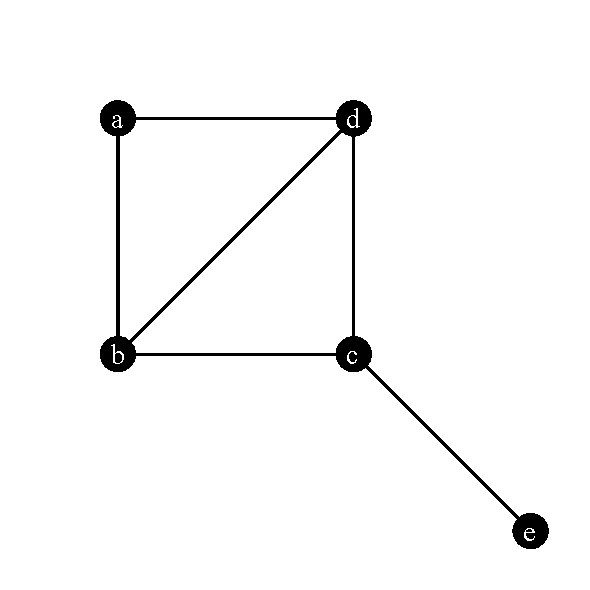
\includegraphics[width=0.8\columnwidth,trim={0 0cm 0 0},clip]{../notebooks/fig1.pdf}}
        \caption{}
    \end{subfigure}%
    ~
    \begin{subfigure}[t]{0.4\textwidth}
        \centering
    \centerline{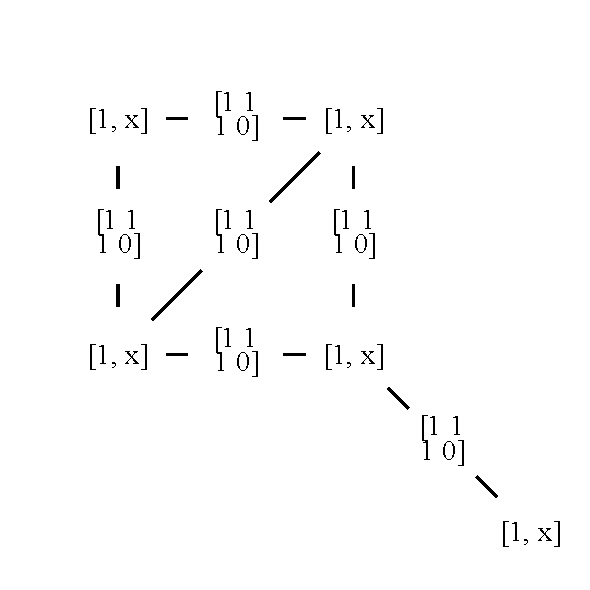
\includegraphics[width=0.8\columnwidth,trim={0 0cm 0 0},clip]{../notebooks/fig2.pdf}}
        \caption{}
    \end{subfigure}
    \caption{Mapping a graph to an einsum network.}\label{fig:einsummapping}
\end{figure*}
The benefit of mapping the problem to einsum is, some existing algorithms can be used to decrease the complexity of the problem.
Especially those techiniques developed in recent quantum circuit simulations for finding the optimal exactly contraction order of a tensor network ~\cite{Gray2021,Pan2021}.
With these algorithms, one can easily find a good contraction order that reduces the complexity to a quantity related to the minimum treewidth of the graph.~\cite{Markov2008}
Such mapping also makes it possible to utilize faster BLAS functions.

Before contracting the tensor network and evaluating this polynomial numerically, let us give up thinking $0$s and $1$s in tensors $W(x)$ and $B$ as regular computer numbers such as integers and floating point numbers.
Instead, we treat them as the additive identity and multiplicative identity of a commutative semiring.
A commutative semiring can be defined as: a ring without additive inverse is called a semiring, and commutative semiring is a semiring that multiplication commutative.

\subsection{Symbolic computing}
To evaluate this polynomial, one can use the symbolic computing directly.
One can store a polynomial of $x$ as a vector of factors.
We define the algebra between the polynomial expansions of order $k$ as
\begin{align}
    \begin{split}
    a \oplus b &= \{a_0 + b_0, a_1 + b_1, \ldots, a_k + b_k\},\\
    a \odot b &= \{a_0 + b_0, a_1b_0 + a_0b_1, \ldots, a_k + b_k\},\\
    \mymathbb{0} &= \{\},\\
    \mymathbb{1} &= \{1\},
    \end{split}
\end{align}
and insert them to the original tensor network contraction algorithm.
In the program, the multiplication can be evaluated efficiently with the convolution theorem.
However, this method still suffers from a space overhead that propotional to the maximum independant set size.

\subsection{Polynomial fitting}
Let $m$ be the maximum independent set size and $X$ be a set of $m+1$ random real numbers, e.g. $\{0, 1, 2, \ldots, m\}$.
We compute the einsum contraction for each $x \in X$ and obtain the following relations
\begin{align}
    \begin{split}
a_0 + a_1 x_1 + a_1 x_1^2 + \ldots + a_m x_1^m &= y_0\\
a_0 + a_1 x_2 + a_2 x_2^2 + \ldots + a_m x_2^m &= y_1\\
\ldots&\\
a_0 + a_1 x_m + a_2 x_m^2 + \ldots + a_m x_m^m& = y_m
    \end{split}
\end{align}
The polynomial fitting between $X$ and $Y = \{y_0, y_1, \ldots, y_m\}$ gives us the factors.

\subsection{Fourier transformation}
\begin{align}
\left(\begin{matrix}
1 & x_1 & x_1^2 & \ldots & x_1^m \\
1 & x_2 & x_2^2 & \ldots & x_2^m \\
\vdots & \vdots & \vdots &\ddots & \vdots \\
1 & x_m & x_m^2 & \ldots & x_m^m
\end{matrix}\right)
\left(\begin{matrix}
a_0 \\ a_1 \\ \vdots \\ a_m
\end{matrix}\right)
= \left(\begin{matrix}
y_0 \\ y_1 \\ \vdots \\ y_m
\end{matrix}\right)
\end{align}

\begin{align}
\left(\begin{matrix}
1 & r\omega & r^2\omega^2 & \ldots & r^m\omega^m \\
1 & r\omega^2 & r^2\omega^4 & \ldots & r^m\omega^{2m} \\
\vdots & \vdots & \vdots &\ddots & \vdots \\
1 & r\omega^m & r^2\omega^{2m} & \ldots & r^m\omega^{m^2}
\end{matrix}\right)
\left(\begin{matrix}
a_0 \\ a_1 \\ \vdots \\ a_m
\end{matrix}\right)
= \left(\begin{matrix}
y_0 \\ y_1 \\ \vdots \\ y_m
\end{matrix}\right)
\end{align}

When $r=1$, the left side is a DFT matrix. We can obtain the factors using the relation $\vec a = {\rm FFT^{-1}}(\omega) \cdot \vec y$.
In the special case that $\omega = e^{-2\pi i/(m+1)}$, it is directly solvable with inverse fast fourier transformation algorithm in package \texttt{FFTW}.

\begin{equation}
{\rm FFT}(\omega) \cdot \vec a_r = \vec y
\end{equation}
where $(\vec a_r)_k = a_k r ^k$, by choosing diferent $r$, we can obtain better precision in low independant set size region  ($\omega<1$) and high independant set size region ($\omega>1$).

\subsection{Finite field algebra}
It is possible to compute the independence polynomials exactly using basic integer types only,
even when the degeneracy is bigger than that can be represented by 64 bit integers.
What we need is computing with the finite field algebra $GF(p)$

\begin{align}
\begin{split}
    x\pmod p ~\oplus~ y\pmod p &= x+y\pmod p\\
    x\pmod p ~\odot~ y\pmod p &= xy\pmod p\\
    \mymathbb{0} &= 0\\
    \mymathbb{1} &= 1
\end{split}
\end{align}

It a field because the multiplicative inverse can defined on non-zero values, which can be computed with the extended Euclidean algorithm.
In a finite field algebra, we have the following observations
\begin{enumerate}
    \item One can still use Gaussian elimination~\cite{Golub2013} to solve the linear equations in a finite field, since the multiplicative inverse is properly defined in a finite field,
    \item Let remainders of an integer $x$ over a set of coprime integers $\{p_1, p_2, \ldots, p_n\}$ being $\{x \pmod {p_1}, x\pmod {p_2}, \ldots, x \pmod {p_n}\}$,
    then $\{x \pmod {p_1 \times p_2 \times \ldots \times p_n}\}$ can be obtained using the chinese remainder theorem.
\end{enumerate}
With these observations, we use Algorithm~\ref{alg:finitefield} to compute degeneracies.
In the algorithm, except the computation of chinese remainder theorem, all computations are done with integers with fixed width.

\begin{algorithm}[!ht]
    \small
    \SetAlgoNoLine
    \LinesNumbered
    Let $P = 1$, $X = {0,1,2,\ldots,m}$ and $\hat X_{ij} = X_i^j$, where $i,j = \{0, 1, \ldots m\}$\;
    \While{true}{
        compute the largest prime 64 bit integer $p$ that $\gcd(p, P) = 1$\;
        compute the tensor network contraction on $GF(p)$ and obtain $Y\pmod p = \{y_0 \pmod p, y_1 \pmod p, \ldots , y_m \pmod p\} $\;
        $A \pmod p = \{a_0 \pmod p, a_1 \pmod p, \ldots, a_m \pmod p\} = {\rm gaussian\_elimination}(\hat X, Y \pmod p) $\;
        $A \pmod {P\times p} = {\rm chinese\_remainder}(A \pmod P, A \pmod p)$\;
        \If{$A \pmod P = A \pmod {P \times p}$}{
            \Return $A \pmod P$\;
        }
        $P = P \times p$\;
    }\caption{Compute independence polynomial exactly without integer overflow}\label{alg:finitefield}
\end{algorithm}

\section{Computing maximum independent set size and its degeneracy}
Obtaining the maximum independent set size and its degeneracy is much easier. Let $x=\infty$, then the independence polynomial becomes
\begin{equation}
I(G, \infty) = a_k \infty^{\alpha(G)},
\end{equation}
where the lower orders terms disappear automatically. We can define a new algebra as
\begin{align}
\begin{split}
    a_x\infty^x \oplus a_y\infty^y &= \begin{cases}
        (a_x + a_y)\infty^{\max(x,y)}, & x = y\\
        a_y\infty^{\max(x,y)}, & x < y\\
        a_x\infty^{\max(x,y)}, & x > y
    \end{cases}\\
    a_x\infty^x \odot a_y\infty^y &= a_x a_y\infty^{x+y}\\
    \mymathbb{0} &= -\infty\\
    \mymathbb{1} &= 0
\end{split}
\end{align}
In the program, we only store the power $x$ and the corresponding factor $a_x$ that initialized to $1$. This is exactly the tropical tensor network~\cite{Liu2021} used in solving spin glass ground states.
Here if we are only interested in obtaining $\alpha(G)$, we can only consider the powers, which corresponds to the tropical algebra~\cite{Maclagan2015}.

One may want to obtain all ground state configurations,
it can be achieved replacing the factors $a_x$ with a set of bit strings $s_x$ initialized to a vertex dependent value $s_i = \{\delta_{ij=1,\ldots,n}$\}.
The bit strings has a redefined algebra
\begin{align}
\begin{split}
    s_x \oplus s_y &= s_x \cup s_y\\
    s_x \odot s_y &= \{\sigma \lor \tau | \sigma \in s_x, \tau \in s_y\}
\end{split}
\end{align}
The $\vee$ is the bit-wise \texttt{or}.

\subsection{Utilizing sparsity}
So far, we have used the language of einsum networks for contraction.
When using sparse tropical tensor networks to find the maximum independent set, we can introduce a new rule to compress the tensor by removing elements that are not helpful.
As show in \Fig{fig:compressrule}, after we contract the tensors in a subregion $R \subseteq G$ of a graph $G$, and obtain a resulting tensor $A$ of rank $|C|$, where $C$ is the set of vertice tensors at the cut.
Each tensor entry $A_{\sigma}$ defines a local maximum independant set size with a fixed boundary configuration $\sigma \in \{0,1\}^{|C|}$ by marginalizing the inner degrees of freedom.
We call this properly the \textit{local maximum rule}.

In addition, suppose we have two entries with the same local maximum independent set size corresponding to local configurations shown in (a) and (b), it is safe to claim configuration (a) being better than configuration (b) and remove the entry $A_{\sigma_b}$.
This is because the boundary of (a) is less restrictive to the rest of the graph while having the equally good local maximum independent set size, 
i.e. any exterior configuration $\overline{\sigma}$ making $\overline{\sigma} \cup \sigma_b$ a global maximum independent set also makes $\overline{\sigma} \cup \sigma_a$ a maximum independent set.
Hence an entry $A_{\sigma_a}$ is ``better'' than $A_{\sigma_b}$ can be defined as
\begin{align}
(\sigma_a \land \sigma_b = \sigma_a) \land (A_{\sigma_a} \geq A_{\sigma_b}),\label{eq:compress}
\end{align}
where $\land$ is a bitwise and operations.
The first term means that whenever a bit in $\sigma_a$ has boolean value $1$, the corresponding bit in $\sigma_b$ is also $1$.
While the second term means the maximum independant set size with boundary configuration fixed to $\sigma_a$ is not less than that fixed to $\sigma_b$.
The word ``better'' means the best solution with boundary configuration $\sigma_a$ is never worse than that with $\sigma_b$.
When Eq. \ref{eq:compress} holds, It is easy to see that if $\sigma_b \cup \overline{\sigma_b}$ is one of the solutions for maximum independant sets in $G$, $\sigma_a \cup \overline{\sigma_b}$ is also a solution.
With this observation, it is safe to set $A_{\sigma_b}$ to tropical zero.
We call this property the \textit{least restrictive rule}, that is,
among boundary configurations with equal local maximum independent sizes,
we only retain those least restrictive (less ones at the boundary) to exterial configurations.

\begin{figure}
    \centering
    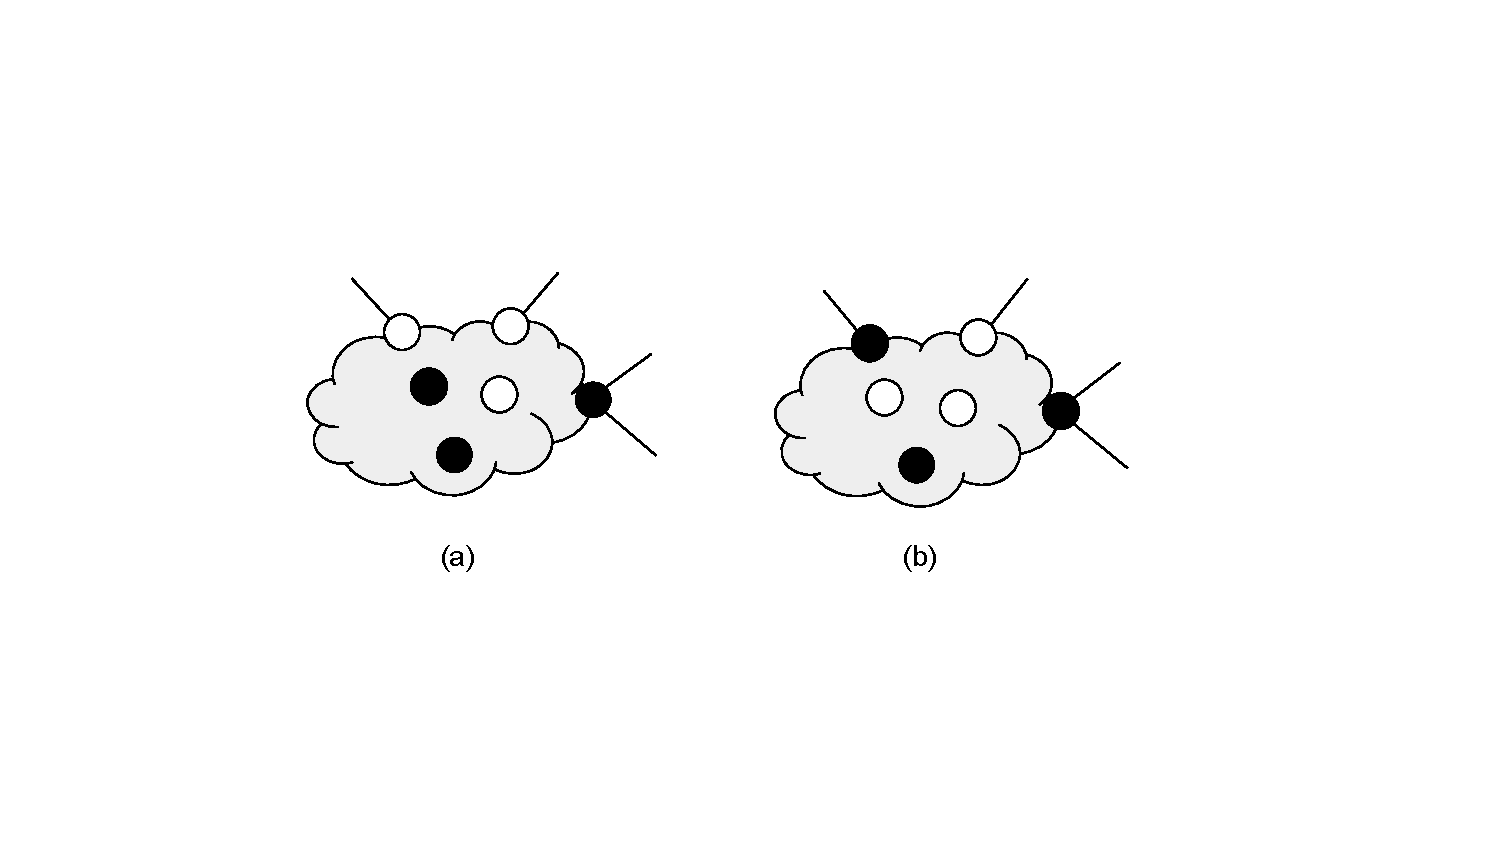
\includegraphics[width=0.8\textwidth, trim={5cm 4cm 5cm 4cm}, clip]{compressionrule.pdf}
    \caption{Two configurations with same local independent size $v_a = v_b = 3$ and different boundary configurations (a) ${001}$ and (b) ${101}$, where black nodes are $1$s (in the independent set) and white nodes are $0$s (not in the independent set).}\label{fig:compressrule}
\end{figure}

\subsection{The tensor network compression detects branching rules automatically}
In the following, we are going to show \textit{local maximum rule} and \textit{least restrictive rule} can automatically discover branching rules and use it for compressing tensor elements,
i.e. sparse tropical tensor network can not be worse than branching in truncating the search space.

We are going the verify the Lemmas used for branching in book~\cite{Fomin2013}.
\begin{theorem}\label{rule:one} % basic
  If a vertex $v$ is in an independent set $I$, then none of its neighbors can be in $I$.
On the other hand, if $I$ is a maximum (and thus maximal) independent set,
and thus if $v$ is not in $I$ then at least one of its neighbors is in $I$.
\end{theorem}

Contract $N[v]$ and the resulting tensor $A$ has a rank $|N(v)|$. Each tensor entry $A_{\sigma}$ corresponds to a locally maximized independant set size with fixed boundary configuration $\sigma \in \{0, 1\}^{|N(v)|}$.
If the boundary configuration is a bit string of 0s, $\sigma_v$ will takes value $1$ to maximize the local independant set size.

\begin{theorem} % 2.5
Let $G=(V,E)$ be a graph, let $v$ and $w$ be adjacent vertices of $G$ such that $N[v] \subseteq N[w]$. Then
\begin{equation}
\alpha(G)=\alpha(G\backslash w).
\end{equation}
\end{theorem}

Contract $N[w]$, both $\{v, w\}$ disapear from the tensor indices because they are inner degrees of freedom.
If $w$ is one, then $N[v]$ are all zeros, the resulting tensor element can not be larger than setting $v=1$ and $w=0$.
By the maximization rule, the local tensor does not change if we remove $w$.

\begin{theorem} % 2.6
  Let $G = (V, E)$ be a graph and let $v$ be a vertex of $G$. If no maximum
independent set of $G$ contains $v$ then every maximum independent set of $G$ contains
at least two vertices of $N(v)$.
\end{theorem}
Contract $N[v]$, the minimum tensor element is $2$, otherwise letting $v$ be in the independent set is one of the solutions. This is again captured by the \textit{local maximum rule}.

\begin{theorem} % 2.7
Let $G = (V, E)$ be a graph and $v$ a vertex of $G$. Then
\begin{equation}
\alpha(G) = \max(1 + \alpha(G \backslash N[v]), \alpha(G \backslash (M(v) \cup \{v\})).
\end{equation}
\end{theorem}

Here, $M(v)$ is the set of mirrors of $v$ in $G$.
A vertex $w \in N^2(v)$ is called a mirror of $v$ if $N(v) \backslash N(w)$ is a clique.
This rule states that if $v$ is not in $M$, there exists an MIS $I$ that $M(v)\notin I$.
otherwise, there must be one of $N(v)$ in the MIS (\textit{local maximum rule}).
If $w$ is in $I$, then none of $N(v) \cap N(w)$ is in $I$, then there must be one of node in the clique $N(v)\backslash N(w)$ in $I$ (\textit{local maximum rule}),
since clique has at most one node in the MIS, the tensor compression will eliminate this solution by moving the occuppied node to the interior.
Hence, the \textit{least restrictive rule} captures the mirror rule.

\begin{theorem} % 2.9
Let $G = (V, E)$ be a graph and $v$ be a vertex of $G$ such that $N[v]$ is a
clique. Then
\begin{equation}
\alpha(G) = 1 + \alpha(G \backslash N[v]).
\end{equation}
\end{theorem}

Contract $N[v]$, and this rule can be captured by the \textit{local maximum rule}.

\begin{theorem}  %2.10
Let $G$ be a graph, let $S$ be a separator of $G$ and let $I(S)$ be the set of
all subsets of $S$ being an independent set of $G$. Then
\begin{equation}
\alpha(G) = \max_{A\in I(S)} |A| + \alpha(G \backslash (S \cup N[A])).
\end{equation}
\end{theorem}
This rule corresponds to first contract tensors in subgraph $S$, then $N[S]$, and then contract the rest parts.
These branching rule can be captured by the \textit{local maximum rule}.

\begin{theorem}  %2.11
Let $G = (V, E)$ be a disconnected graph and $C \subseteq V$ a connected component of $G$. Then
\begin{equation}
\alpha(G) = \alpha(G[C]) + \alpha(G \backslash C)).
\end{equation}
\end{theorem}
Contract by the disconnected parts, and this rule can be captured by the \textit{local maximum rule}.

\iffalse
\begin{align}
if |V| = 0 then
return 0
if \exists v \in V with d(v) \leq 1 then
return 1 + mis2(G \backslash N[v])
if \exists v \in V with d(v) = 2 then
(let u 1 and u 2 be the neighbors of v)
if {u 1 , u 2 } \in E then
return 1 + mis2(G \backslash N[v])
if {u 1 , u 2 } \in
/ E then
if |N 2 (v)| = 1 then
(let N 2 (v) = {w})
return max(2 + mis2(G \backslash (N 2 [v] \cup N[w])), 2 + mis2(G \backslash N 2 [v]))
if |N 2 (v)| > 1 then
return max(mis2(G \backslash N[v]), mis2(G \backslash (M(v) \cup cup))
if \exists v \in V with d(v) = 3 then
(let u 1 u 2 and u 3 be the neighbors of v)
if G[N(v)] has no edge then
if v has a mirror then
return max(1 + mis2(G \backslash N[v]), mis2(G \backslash (M(v) \cup {v}))
if v has no mirror then
return max(1 + mis2(G \backslash N[v]), 2 + mis2(G \backslash N[{u 1 , u 2 }]), 2 + mis2(G \backslash
(N[{u_1 , u_3 }] \cup \{u_2\})), 2 + mis2(G \backslash (N[{u_2 , u_3 }] \cup \{1\})))
if G[N(v)] has one or two edges then
return max(1 + mis2(G \backslash N[v]), mis2(G \backslash (M(v) \cup cup))
if G[N(v)] has three edges then
return 1 + mis2(G \backslash N[v])
if \Delta (G) \geq 6 then
choose a vertex v of maximum degree in G
return max(1 + mis2(G \backslash N[v]), mis2(G \backslash v))
if G is disconnected then
(let C \subseteq V be a component of G)
return mis2(G[C]) + mis2(G \backslash C)
if G is 4 or 5-regular then
choose any vertex v of G
return max(1 + mis2(G \backslash N[v]), mis2(G \backslash (M(v) \cup \{v\}))
if \Delta (G) = 5 and \delta (G) = 4 then
choose adjacent vertices v and w with d(v) = 5 and d(w) = 4 in G
return
\max(1 + mis2(G \backslash N[v]), 1 + mis2(G \backslash (\{v\} \cup M(v) \cup N[w])), mis2(G \backslash (M(v) \cup \{v, w\})))
\end{align}
\fi

\bibliographystyle{iclr2021_conference}
\bibliography{refs}

\appendix

\section{Technical guide}
\begin{description}
	\item[OMEinsum] a package for einsum,
	\item[OMEinsumContractionOrders] a package for finding the optimal contraction order for einsum \\ \href{https://github.com/Happy-Diode/OMEinsumContractionOrders.jl}{https://github.com/Happy-Diode/OMEinsumContractionOrders.jl},
	\item[TropicalGEMM] a package for efficient tropical matrix multiplication (compatible with OMEinsum),
	\item[TropicalNumbers] a package providing tropical number types and tropical algebra, one o the dependency of TropicalGEMM,
	\item[LightGraphs] a package providing graph utilities, like random regular graph generator,
	\item[Polynomials] a package providing polynomial algebra and polynomial fitting,
	\item[Mods and Primes] packages providing finite field algebra and prime number generators.
\end{description}

One can install these packages by opening a julia REPL, type \colorbox{lightgray}{\texttt{]}} to enter the \texttt{pkg>} mode and type, e.g.
\begin{lstlisting}
pkg> add OMEinsum
\end{lstlisting}

An example of computing the maximum independant set size
\begin{lstlisting}
julia> using OMEinsum, LightGraphs, TropicalNumbers

julia> n, k = 6, 3
(6, 3)

julia> g = LightGraphs.random_regular_graph(n, k)
{6, 9} undirected simple Int64 graph

julia> ixs = [minmax(e.src,e.dst) for e in LightGraphs.edges(g)]
9-element Vector{Tuple{Int64, Int64}}:
 (1, 2)
 (1, 4)
 (1, 5)
 (2, 3)
 (2, 6)
 (3, 5)
 (3, 6)
 (4, 5)
 (4, 6)

julia> code = EinCode((ixs..., [(i,) for i in LightGraphs.vertices(g)]...), ())
1∘2, 1∘4, 1∘5, 2∘3, 2∘6, 3∘5, 3∘6, 4∘5, 4∘6, 1, 2, 3, 4, 5, 6 -> 

julia> optimized_code = optimize_greedy(code, Dict([i=>2 for i=1:6]))
4∘6, 4∘6 -> 
├─ 4∘6, 6 -> 4∘6
│  ├─ 6
│  └─ 4∘6
└─ 2∘5∘4, 5∘2∘6 -> 4∘6
   ├─ 2∘5∘6, 6∘2 -> 5∘2∘6
   │  ├─ 2∘6, 2 -> 6∘2
   │  │  ├─ 2
   │  │  └─ 2∘6
   │  └─ 2∘3, 5∘6∘3 -> 2∘5∘6
   │     ├─ 3∘5, 6∘3 -> 5∘6∘3
   │     │  ├─ 3∘6, 3 -> 6∘3
   │     │  │  ⋮
   │     │  │  
   │     │  └─ 3∘5, 5 -> 3∘5
   │     │     ⋮
   │     │     
   │     └─ 2∘3
   └─ 2∘4∘1, 1∘4∘5 -> 2∘5∘4
      ├─ 1∘5, 5∘4 -> 1∘4∘5
      │  ├─ 4∘5, 4 -> 5∘4
      │  │  ├─ 4
      │  │  └─ 4∘5
      │  └─ 1∘5
      └─ 2∘1, 1∘4 -> 2∘4∘1
         ├─ 1∘4
         └─ 1∘2, 1 -> 2∘1
            ├─ 1
            └─ 1∘2


julia> function mis_contract(code::OMEinsum.NestedEinsum, x::T) where T
           tensors = map(OMEinsum.getixs(Iterators.flatten(code))) do ix
               @assert length(ix) == 1 || length(ix) == 2
                           length(ix) == 1 ? [one(T), x] : [one(T) one(T); one(T) zero(T)]
           end
           code(tensors...)
       end
mis_contract (generic function with 1 method)

julia> result = mis_contract(optimized_code, Tropical(1.0))
0-dimensional Array{TropicalF64, 0}:
2.0ₜ
\end{lstlisting}

For larger graph, we hight recommend using two additional packages,
\texttt{TropicalGEMM} for BLAS speed tropical matrix multiplication and
\texttt{OMEinsumContractionOrders} for hyper optimized contraction order (the KaHyPar~\cite{Schlag2020} approach) ~\cite{Kourtis2019,Gray2021,Pan2021}.


\end{document}
